\documentclass[landscape]{article}
\usepackage[pdftex]{graphicx}
\pagestyle{empty}
\oddsidemargin  -0.5 in
\evensidemargin -0.5 in
\headheight     0 in
\topmargin      -1 in
\textheight     7.7 in
\textwidth      10 in
\begin{document}
\huge
\renewcommand{\labelitemi}{-}
\setlength{\parindent}{0 cm}

All the publicity plots for $\chi_{1 \mbox{\large or } 2}^0 \, \chi_3^0 \to$ two leptons:

\vfill

\begin{center} \begin{tabular}{p{0.45\linewidth} p{0.45\linewidth}}
    \includegraphics[width=\linewidth]{again1.pdf} &
    \includegraphics[width=\linewidth]{again2.pdf}
\end{tabular} \end{center}

\vfill

Only one cut: missing energy $>$ 350 GeV.  Polarization, as well as
adding like and subtracting unlike flavors, does the rest.

\vfill

Constraint on cross-sections: $0.01335 \, \sigma_{13} + 0.00580 \, \sigma_{23} = 1 \pm 0.059 \, \sqrt{\frac{250 \mbox{ \large fb}^{-1}}{\mbox{\large int lumi}}}$

\vfill

Edge resolution is 0.7 GeV with 250 fb$^{-1}$ and 2 GeV with 50
fb$^{-1}$, but will require a more sophisticated fitting technique to
be unbiased.

\pagebreak

\mbox{ }

\vfill

Can we extract the LSP mass from two leptons?

\vfill

\begin{center} \begin{tabular}{p{0.45\linewidth} p{0.45\linewidth}}
    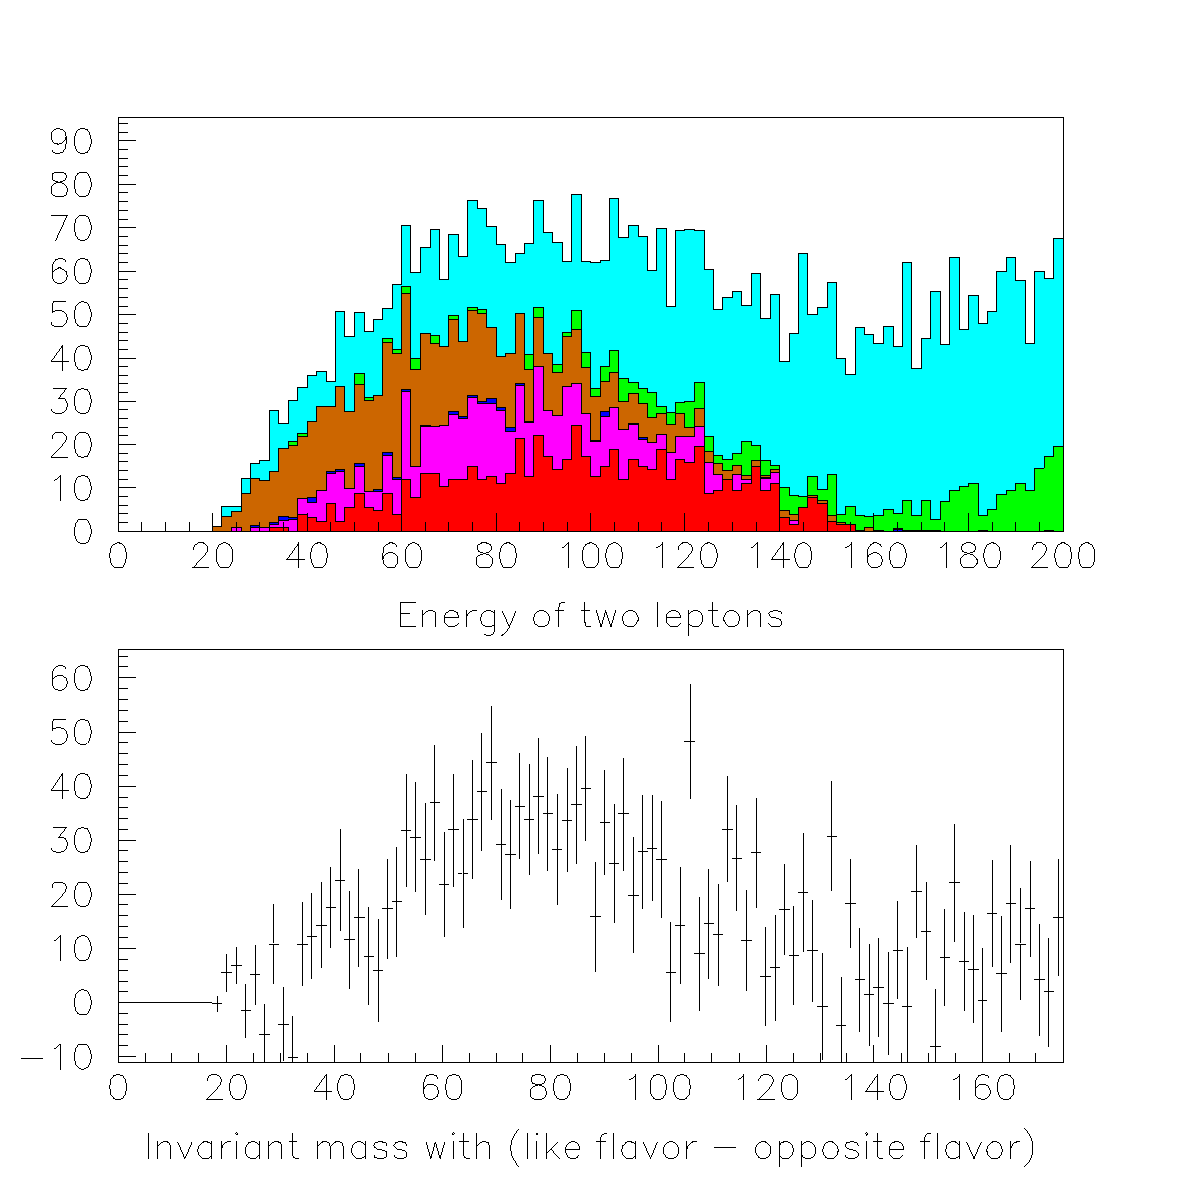
\includegraphics[width=\linewidth]{again_energy_nocut.pdf} &
    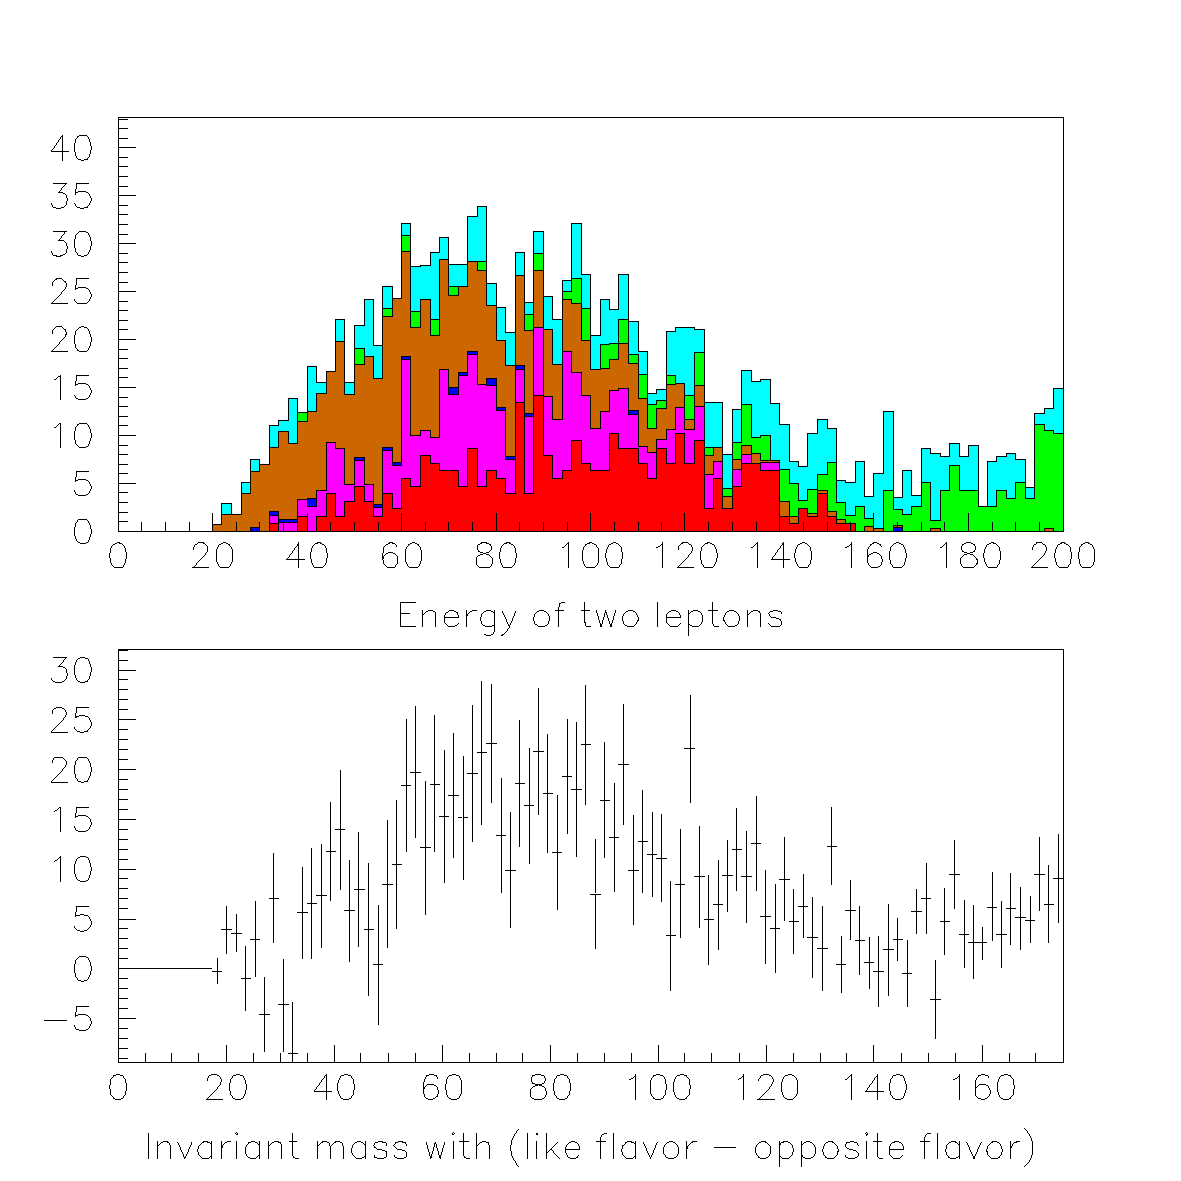
\includegraphics[width=\linewidth]{again_energy_withcut.pdf}
\end{tabular} \end{center}

\vfill

The plots on the right feature a $W^+W^-$-suppressing anglular cut.

\vfill

\mbox{ }

\end{document}
